% note: no \documentclass{} - this file is included from burntalk-*.tex
\usepackage{tikz}
\usepackage{graphicx}
\usepackage{pgffor}
\usepackage{xspace}
\usepackage{comment}
\usepackage[rel]{overpic}
\usepackage{hyperref}

\graphicspath{{./figures/} {./patfigs/}}

% \imseq{preceding text}{sequence name}{sequence}
\newcounter{turncnt}
\newcommand{\theturn}{\arabic{turncnt}}
\newcommand{\imseq}[3]{%
	\foreach \n [count=\sliden] in {#3}{%
		\setcounter{turncnt}{\n}%
		\addtocounter{turncnt}{1}%
		\only<\sliden>{%
		\centering%
		#1%
		\parbox[t][0.6\paperheight][c]{\textwidth}{%
			\begin{center}%
				\includegraphics[height=0.6\textheight,width=0.8\textwidth,keepaspectratio]{#2-\n.eps}%
			\end{center}
			}%
		}%
	}%
}
% \countseq{preceding text}{sequence name}{count}
\newcommand{\countseq}[3]{\imseq{#1}{#2}{0,...,#3}}
% \gametext
\newcommand{\gametext}{Turn \theturn\\\medskip}
% \game{sequence name}{count}
\newcommand{\game}[2]{\countseq{\gametext}{#1}{#2}}
% \on
%\newcommand{\on}[0]{\textcolor{orange}{\bf on}}
\newcommand{\on}[0]{\textcolor{orange}{\bf 1}\xspace}
% \off
%\newcommand{\off}[0]{off}
\newcommand{\off}[0]{0\xspace}

% \qmark
\newcommand{\qmark}[0]{{\large ?}}
% \rqmark
\newcommand{\rqmark}[0]{\textcolor{white}{\qmark}}

\title{Computation in the game of Life}
\author{Lucas Jones}
\date{February 25, 2015}

\begin{document}

\maketitle

\begin{frame}{The game of Life}{The rules}
	\begin{columns}[onlytextwidth]
		\begin{column}{0.3\textwidth}
			\centering
			\begin{overpic}[width=0.75\textwidth,height=\textheight,keepaspectratio]{rules1-0}
				\put(26,64){\rqmark}
				\put(46,64){\rqmark}
				\put(66,64){\qmark}

				\put(26,44){\qmark}
				\put(46,44){\textcolor{white}{\bf 4}}
				\put(66,44){\qmark}

				\put(26,24){\qmark}
				\put(46,24){\rqmark}
				\put(66,24){\rqmark}
			\end{overpic}

			\medskip
			{\Large $> 3$\\ dies}
		\end{column}
		\begin{column}{0.3\textwidth}
			\centering
			\begin{overpic}[width=0.75\textwidth,height=\textheight,keepaspectratio]{rules2-0}
				\put(26,64){\rqmark}
				\put(46,64){\qmark}
				\put(66,64){\qmark}

				\put(26,44){\qmark}
				\put(46,44){\textcolor{white}{\bf 1}}
				\put(66,44){\qmark}

				\put(26,24){\qmark}
				\put(46,24){\qmark}
				\put(66,24){\qmark}
			\end{overpic}

			\medskip
			{\Large $< 2$\\ dies}
		\end{column}
		\begin{column}{0.3\textwidth}
			\centering
			\begin{overpic}[width=0.75\textwidth,height=\textheight,keepaspectratio]{rules3-0}
				\put(26,64){\rqmark}
				\put(46,64){\rqmark}
				\put(66,64){\qmark}

				\put(26,44){\qmark}
				\put(46,44){\bf 3}
				\put(66,44){\qmark}

				\put(26,24){\qmark}
				\put(46,24){\qmark}
				\put(66,24){\rqmark}
			\end{overpic}

			\medskip
			{\Large $= 3$\\ is born}
		\end{column}
	\end{columns}

	\note[item]{A bit different from other games you've played; invented by John Horton Conway in 1970}
	\note[item]{A zero-player game played on an infinite 2-D grid of squares}
	\note[item]{Every square starts off either alive or dead}
	\note[item]{At start of turn: go through living cells; count neighbours}
	\note[item]{If less than 2, die of isolation}
	\note[item]{If living and greater than 3, die of overcrowding}
	\note[item]{Then dead cells: if 3 live neighbours, born}
\end{frame}

\begin{frame}{The game of Life}{An example}
	\begin{columns}[onlytextwidth]
		\begin{column}{0.3\textwidth}
			\countseq{}{game1}{5}
		\end{column}
		\begin{column}{0.3\textwidth}
			\countseq{}{game2}{5}
		\end{column}
		\begin{column}{0.3\textwidth}
			\countseq{}{game3}{5}
		\end{column}
	\end{columns}

	\note[item]{From these simple rules, complicated and unpredictable behaviour arises}
	\note[item]{We can make sense of the behaviour by looking at individual stable patterns}
	\note[item]{Our aim is to build up a pattern sufficiently complicated that it can do `useful' computation}
	\note[item]{Going to look at some of these small, stable patterns}
\end{frame}

\begin{comment}
\begin{frame}{The game of Life}
%	\begin{itemize}
%		\item Invented by John H. Conway in 1970
%		\item Popularised by Martin Gardner in Scientific American
%	\end{itemize}

	\begin{columns}[onlytextwidth]
	\begin{column}{0.5\textwidth}
		\centering
		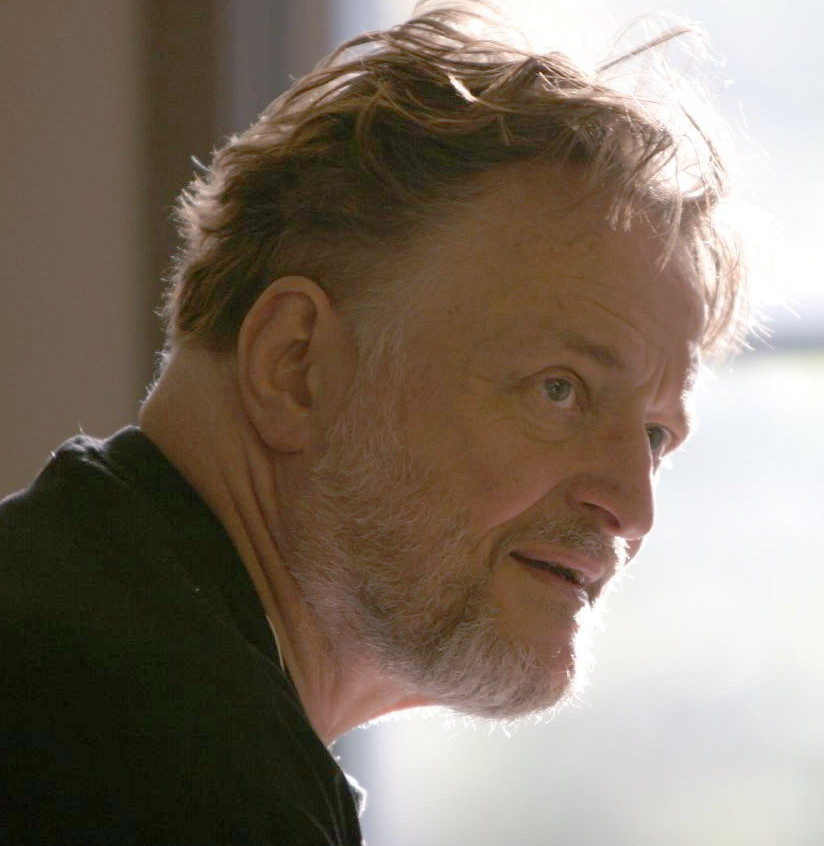
\includegraphics[width=0.9\textwidth]{conway} \\
		John H. Conway
% CC-BY: Thane Plambeck: http://www.flickr.com/photos/thane/20366806/
	\end{column}

	\begin{column}{0.5\textwidth}
		\centering
		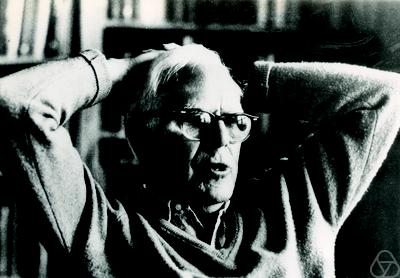
\includegraphics[width=0.9\textwidth]{gardner} \\
		Martin Gardner
% CC-BY-SA: http://owpdb.mfo.de/detail?photo_id=1292
	\end{column}
	\end{columns}
\end{frame}
\end{comment}

\begin{frame}{Some stable patterns}{Still lifes}
	\game{still1}{2}
	Still lifes have period 1.
\end{frame}

\begin{frame}{Some stable patterns}{Blinkers}
	\game{blinker}{3}
	This blinker has period 2.
\end{frame}

\begin{frame}{More complex behaviour}{Gliders}
	\game{glider}{4}
	The glider shape has period 4, but moves from its original position.
\end{frame}

\begin{frame}{More complex behaviour}{Glider versus glider}
	\game{glidervs}{4}
	When two gliders collide, they annihilate each other.
\end{frame}

\begin{comment}
\begin{frame}{How complex can we go?}
% http://ddi.cs.uni-potsdam.de/HyFISCH/Produzieren/lis_projekt/proj_gamelife/ConwayScientificAmerican.htm
	\begin{block}{Conjecture (Conway, 1970)}
		There does not exist a finite initial configuration such that the number of live cells after $n$ turns goes off to infinity.
	\end{block}
	\medskip

%	\pause
%	\begin{itemize}
%		\item Disproved shortly afterwards by Gosper (1970)
%		\item In fact, a much more interesting result was later shown by Conway himself (1982)
%	\end{itemize}
\end{frame}
\end{comment}

% best source I can find for date: http://gosper.org/bill.html
\begin{frame}{How complex can we go?}{Unbounded growth: Gosper's glider gun}
	\imseq{\gametext}{gosper}{0,3,...,42,45}
	The glider gun has period 30, shooting out a glider every cycle.

	\note[item]{Complicated looking thing; discovered by Bill Gosper in 1970}
	\note[item]{Run it through 3 turns at a time; spot the glider on cycle 15}
	\note[item]{As we go through a few, see glider will escape unscathed}
	\note[item]{Getting to another period --- 30 cyles --- we get 2 gliders}
\end{frame}

\begin{frame}{How complex can we go?}
	\pause
% see Rendell (2014)
	\begin{block}{Theorem}
		Life is Turing-complete.
	\end{block}

	\pause
	\begin{center}
		\rotatebox{90}{$\iff$}
	\end{center}

	\begin{block}{Theorem}
		If anything else can compute the result of a given function, so can Life.
	\end{block}
\end{frame}

%\begin{frame}{Logic gates}
%	\begin{itemize}
%		\item Many ways of modelling computation in Life have been discovered
%		\item Modern digital computer chips are built from billions of logic gates
%		\item Constructing logic gates in Life will give us a means to compute things
%	\end{itemize}
%\end{frame}

\begin{frame}{Logic gates}
	\note[item]{Going to use the same logic gate construction Conway used}
	\note[item]{Boolean functions operate on two values: \on and \off}
	\note[item]{Can express all such functions as combinations of $\mathsf{NOT}$ and $\mathsf{AND}$}

	\pause
	\bigskip
	\begin{columns}[onlytextwidth]
		\begin{column}{0.5\textwidth}
			\centering
			\begin{tabular}{c|c}
				$x$ & $\mathsf{NOT}~ x$ \\
				\hline
				\on & \off \\
				\off & \on
			\end{tabular}
		\end{column}

		\begin{column}{0.5\textwidth}
			\centering
			\begin{tabular}{c|c|c}
				$x$ & $y$ & $x ~\mathsf{AND}~ y$ \\
				\hline
				\on & \on & \on \\
				\on & \off & \off \\
				\off & \on & \off \\
				\off & \off & \off
			\end{tabular}
		\end{column}
	\end{columns}

%	\pause
%	\medskip
%	\begin{itemize}
%		\item Any Boolean function can be expressed as a combination of these gates
%		\item We can do binary arithmetic with Boolean functions
%	\end{itemize}
\end{frame}

\begin{comment}
\begin{frame}{Logic gates}{NAND}
	\begin{itemize}
		\item If we glue together an AND gate and then a NOT gate, we get a NAND gate
	\end{itemize}

	\begin{center}
		\begin{tabular}{c|c|c}
			$a$ & $b$ & $a ~\mathsf{NAND}~ b$ \\
			\hline
			\on & \on & \off \\
			\on & \off & \on \\
			\off & \on & \on \\
			\off & \off & \on
		\end{tabular}
	\end{center}

	\pause
	\begin{itemize}
		\item It turns out any Boolean function can also be expressed as a combination of NANDs
	\end{itemize}
\end{frame}

\begin{frame}{Bringing gates to Life}
	\begin{itemize}
		\item Build a `circuit' where gliders act like electrons carrying current
		\item Just like in a real circuit, gliders present represents \on; no glider means \off
		\item We use glider guns as current sources
		\item We can use interactions with other patterns (such as eaters) to selectively destroy gliders and produce \off{}s
	\end{itemize}
\end{frame}
\end{comment}

\begin{frame}{Bringing gates to Life}{Encoding input}
	\note[item]{We encode a series of bits as a line of gliders}
	\note[item]{A glider represents \on}
	\note[item]{We leave a space to represent \off}
	\note[item]{Timing must be perfect: a glider moves 1 cell every 4 turns}

	\begin{center}
		\begin{overpic}[height=0.75\textheight,keepaspectratio]{bitstream-0}
			\put(11.5,82){\Huge \on}
			\put(29,58){\Huge \on}
			\put(47,34){\Huge \off}
			\put(64.5,11){\Huge \on}
		\end{overpic}
	\end{center}
\end{frame}

\begin{frame}{Bringing gates to Life}{The NOT gate}
	\note[item]{A glider gun continually makes gliders aimed so they collide with the input bitstream}
	\note[item]{If the current bit is \on, the gliders annihilate each other, producing \off}
	\note[item]{If it is \off, the glider from the gun can pass, giving \on}

	\begin{center}
		\begin{tikzpicture}
			\draw[->,thick] (-2,2) -- (-0.1,0.5) node[pos=-.2] {Glider gun};
			\draw[->,thick] (4,2) -- (2.1,0.5) node[pos=-.2] {Input bit $x$};
			\draw (0,0) rectangle (2, 1) node[pos=.5] {Collision};
			\draw[->,thick] (1,-0.1) -- (1,-0.75) node[pos=1.5] {NOT $x$};
		\end{tikzpicture}
	\end{center}
\end{frame}

\begin{frame}[t]{Bringing gates to Life}{The AND gate}
	\note[item]{Collide both bitstreams in sequence}
	\note[item]{If both are \on, the \on from input $x$ consumes the gun glider leaving $y$ free to be output}
	\note[item]{If only one is \on, it will consume the gun glider leaving no gliders left as output}
	\note[item]{If both are \off, the gun glider keeps moving in the wrong direction, where it is tidied up by an eater}

	\begin{center}
		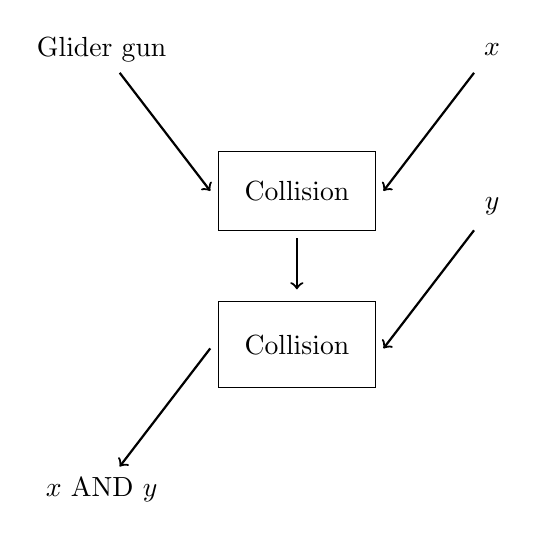
\begin{tikzpicture}
			\draw[->,thick] (-1.25,2) -- (-0.1,0.5) node[pos=-.2] {Glider gun};
			\draw[->,thick] (3.25,2) -- (2.1,0.5) node[pos=-.2] {$x$};
			\draw (0,0) rectangle (2, 1) node[pos=.5] {Collision};
			\draw[->,thick] (1,-0.1) -- (1,-0.75);
			\draw[->,thick] (3.25,0) -- (2.1,-1.5) node[pos=-.2] {$y$};
			\draw (0,-0.9) rectangle (2, -2) node[pos=.5] {Collision};
			\draw[<-,thick] (-1.25,-3) -- (-0.1,-1.5) node[pos=-.2] {$x$ AND $y$};
		\end{tikzpicture}
	\end{center}

	\note[item]{We can embed any finite logic circuit in Life (e.g. a CPU)}
	\note[item]{Can represent the transition function of a Turing machine in this way}
	\note[item]{A combination of gliders and still lifes can act as memory}
	\note[item]{With some machinery, we then have a full Turing machine}
\end{frame}

\begin{frame}{Turing-completeness}
% http://rendell-attic.org/gol/tm.htm
	\note[item]{Rendell (2000) built an `actual' Turing machine pattern in Life}
	\note[item]{Grid dimensions are 1,714~$\times$~1,647}
% http://rendell-attic.org/gol/utm/index.htm
	\note[item]{Rendell later (2010) built a Universal Turing Machine}

	\begin{center}
		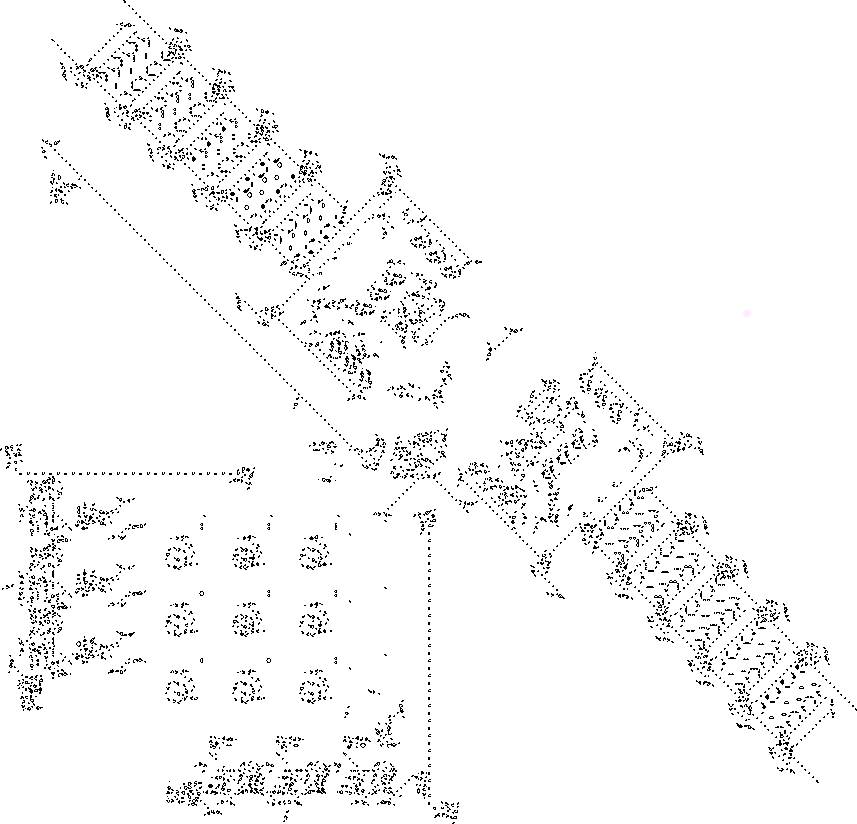
\includegraphics[width=\textwidth,height=0.65\textheight,keepaspectratio]{rendell-tm}

		\medskip
		Rendell's Turing machine \\
		1,714~$\times$~$1,647$
	\end{center}
\end{frame}

\begin{comment}
\begin{frame}{Variations on a theme}
	\begin{itemize}
		\item Life is one of a family of games called `cellular automata'
		\item There are a number of Life-like automata which change the number of neighbours required for a cell to live or die
% http://www.complex-systems.com/pdf/15-1-1.pdf
		\item Cook (2004) showed that even the 1-dimensional Rule 110 automaton is Turing-complete
% http://arxiv.org/abs/1111.1567
		\item Rafler (2011) formulated SmoothLife, a continuous version of Life
	\end{itemize}
\end{frame}
\end{comment}

\end{document}
